\documentclass[12pt, a4paper]{article}
\usepackage[utf8]{inputenc}
\usepackage{hyperref} 
\usepackage{graphicx}
\usepackage[left=2cm, right=2cm, top=2.5cm, bottom=2.5cm]{geometry}
\usepackage{etoolbox}
\patchcmd{\thebibliography}{*}{}{}{}
\graphicspath{ {./images/} }
\title{Predicting slipping weather conditions with decision tree and k-nearest neighbor methods}

\begin{document}
    \maketitle
    \section{Introduction}
    Weather prediction has a key role in our society, but the implications of different weather conditions
    are still mostly up to the human consideration. 
    The current winter has shown that slippery weather might come as a surprise. That is a perfect candidate
    for creating value with weather data.
    
    The goal of this study is to predict slippery conditions on walkways, thus expanding the domain of weather data analysis and prediction. 
    The report consists of problem formulation, model and feature selection, result reporting and conclusions.
    Study suggests a potential machine learning method for the problem and potential further development.
    \section{Problem formulation}
    \subsection{Application of machine learning problem}
    When slippery conditions are expected during the day, a service called \href{https://liukastumisvaroitus.fi/en/}{Liukastumisvaroitus (link)} (Slipping warning) sends subscribers a text-message.

    According to the website, the slippery condition is identified by humans.
    Though one could think that these dangerous weather conditions can be predicted without 
    human knowledge, but to what level of accuracy? This makes it a great target for testing machine learning as an application.
    
    Ideally the machine learning application could predict, given the current weather conditions, whether the slippery warning would be raised.

    The data point is going to be a daily observation of weather data, with the additional
    slippery warning parameter. In other words, a single data point represents the weather conditions of a day. Data includes all data points (daily observations) from around 
    October 2011, as the earliest records of slipping warnings are from then.

    Concluding the parameters, 
    \begin{itemize}
      \item Potential features for the application could be \textit{Precipitation amount}, \textit{Air temperature} and \textit{Snow depth}. All of these properties are numerical and are easily measureable.
      \item The label of the application is going to be whether the \textit{slippery warning} would be raised, with values 0/1.
    \end{itemize}
    
    \section{Methods}

    \subsection{Data sources}
    The slipping warning service offers an API \cite{warnsource} for historical data analysis. Some 600 warnings have been issued in total since October 2011.
    %The slipping warning can be seen to be given at any point during the day, though most usually in the night hours.
    Additionally, the slipping warnings are given on city level for Lahti, Oulu, Kuopio, Jyväskylä, Helsinki, and Joensuu.
    As the slipping warning service data only consists of a timestamp and the city issued, training the machine learning algorithm to account for the current weather conditions needs more data to work with.

    Thus, historical weather data from the Finnish Metheorological Institute \cite{fmisource}
    is combined. Although FMI offers hourly historical data, in this project, the plan is to use the daily aggregated weather recordings for simplicity.
    In total, there are some 3800 (days) * 6 (cities) $\approx$ 23000 daily weather reports since October 2011.
    The FMI data includes air temperature (min/max/overall), ground temperature, precipitation amount and snow depth, which can be used as features in this project.

    Combined together based on the city and the date value, these data sources will be used to train and validate the machine learning algorithm. 
    The labels and features are extracted from the sources and used as explained in the \hyperlink{section.0.2.1}{problem formulation section}. 
    In total we get some 23000 data points for the machine learning application.

    \subsection{Feature selection}
    When you think what causes the most dangerous slipping conditions outside, two conditions need to apply:
    \begin{itemize}
      \item There need to be ice on the road.
      \item There need to be water on the road.
    \end{itemize}
    These conditions are the result of a weather which is around 0°C in temperature and the environment is snowy or waterfall is happening.
    Thus, features selected are \textbf{Air temperature}, \textbf{Maximum temperature}, \textbf{Precipitation amount} and \textbf{Snow depth}. Empirical feature analysis 
    and comparison using my machine learning script and Excel back up these selections. 

    Feature candidates, such as Ground level minimum temperature, were cut off due to lack of data.
    As slipping conditions occur more often when there is snow to be melted away than when ice is forming, maximum temperature can
    suggest better than minimum temperature. Minimum temperature was then left out from the features after analysis.

    \subsection{Models}
    As the machine learning problem is clearly of a classification type, I chose a classification model.
    After analysing different models, I ended up with two potential final alternatives: k-nearest neighbors and decision tree
    classifier. These were chosen based on performance metrics.
  
    \subsubsection{K-nearest neighbors}
    KNN algorithm looks at closest k data points
    to the classification target point and determines the class based on which classes have advantage of prevalence in the area.
    Since there seems to be slim boundaries in the weather metrics when issuing a slipping warning or not, the nearest neighbor
    algorithm can identify even the smallest variations and hopefully lead to good results.

    \subsubsection{Decision tree classifier}
    A decision tree is constructed based on the features given to the model. Classifier organizes the tree and computes
    the most optimal thresholds for decision making.
    Decision tree classifier is suitable for complex classification, which should help in this project, as the
    boudaries in issuing a slipping warning are slim.
    
    \subsubsection{Model selection}
    The selection of the most optimal model will be made using hyperparameter tuning. That is, empirically training and validating different models
    in the hypothesis spaces. For this project, two parameters will be iterated: amount of neighbors and the tree depth will 
    be iterated (from 1 to 32). The results are then analysed by looking at the best validation scores. \autoref{fig:stats} and \hyperlink{section.0.4}{Results section}
    visualize the decision making to a greater detail.

    \subsubsection{Loss function}
    By course material, 0/1 loss is considered the default loss function for especially the k-nearest neighbors classification model. Thus, it is a 
    good starting point for evaluating the model performance and it was chosen as the loss function in this phase. It gives a 
    simple enough performance figure, essentially measuring the accuracy of classification (also function \textit{accuracy\_score} from sklearn).
    
    For Decision tree classifier, the default loss function Gini impurity was used. Changing it to the other alternative,
    information gain, did not make a difference in performance so there was no reason to complicate the model, and the default one was used.

    For validating performance, a combination of accuracy, recall and precision was used. The different statistics
    represent different viewpoints of the model performance, so looking only at one metric would be detrimental. Following
    metrics were selected, as the amount of slipping warnings is low compared to the actual weather observations (600 $<$ 23000). Accuracy gives
    the overall classification correctness. Recall gives what propotion of true slipping warnings were classified correctly.
    Precision gives what propotion of classified slipping warnings were correct. 
    \subsection{Data set construction}
    As the amount of slipping warnings is quite low compared to the actual weather observations (600 $<$ 23000), performing a random split once might lead to 
    very polarised results regarding the contained warnings. Thus, k-fold approach is used to mitigate the random split variations better.

    Training and validation data is splitted with the k-fold approach. K-fold runs the training and validation cycle multiple times for different
    subsets of the data. Data consists of some 23000 data points, which is splitted in to 5 folds as it is the default in the sklearn utility. 
    Folding 5 times results in a training set of 18000 data points and a validation set of 5000 data points in each run.
    
    \section{Results}
    \begin{figure}
      \caption{Graphs comparing different parameters of KNN and decision tree methods}\label{fig:stats}
      \centering
      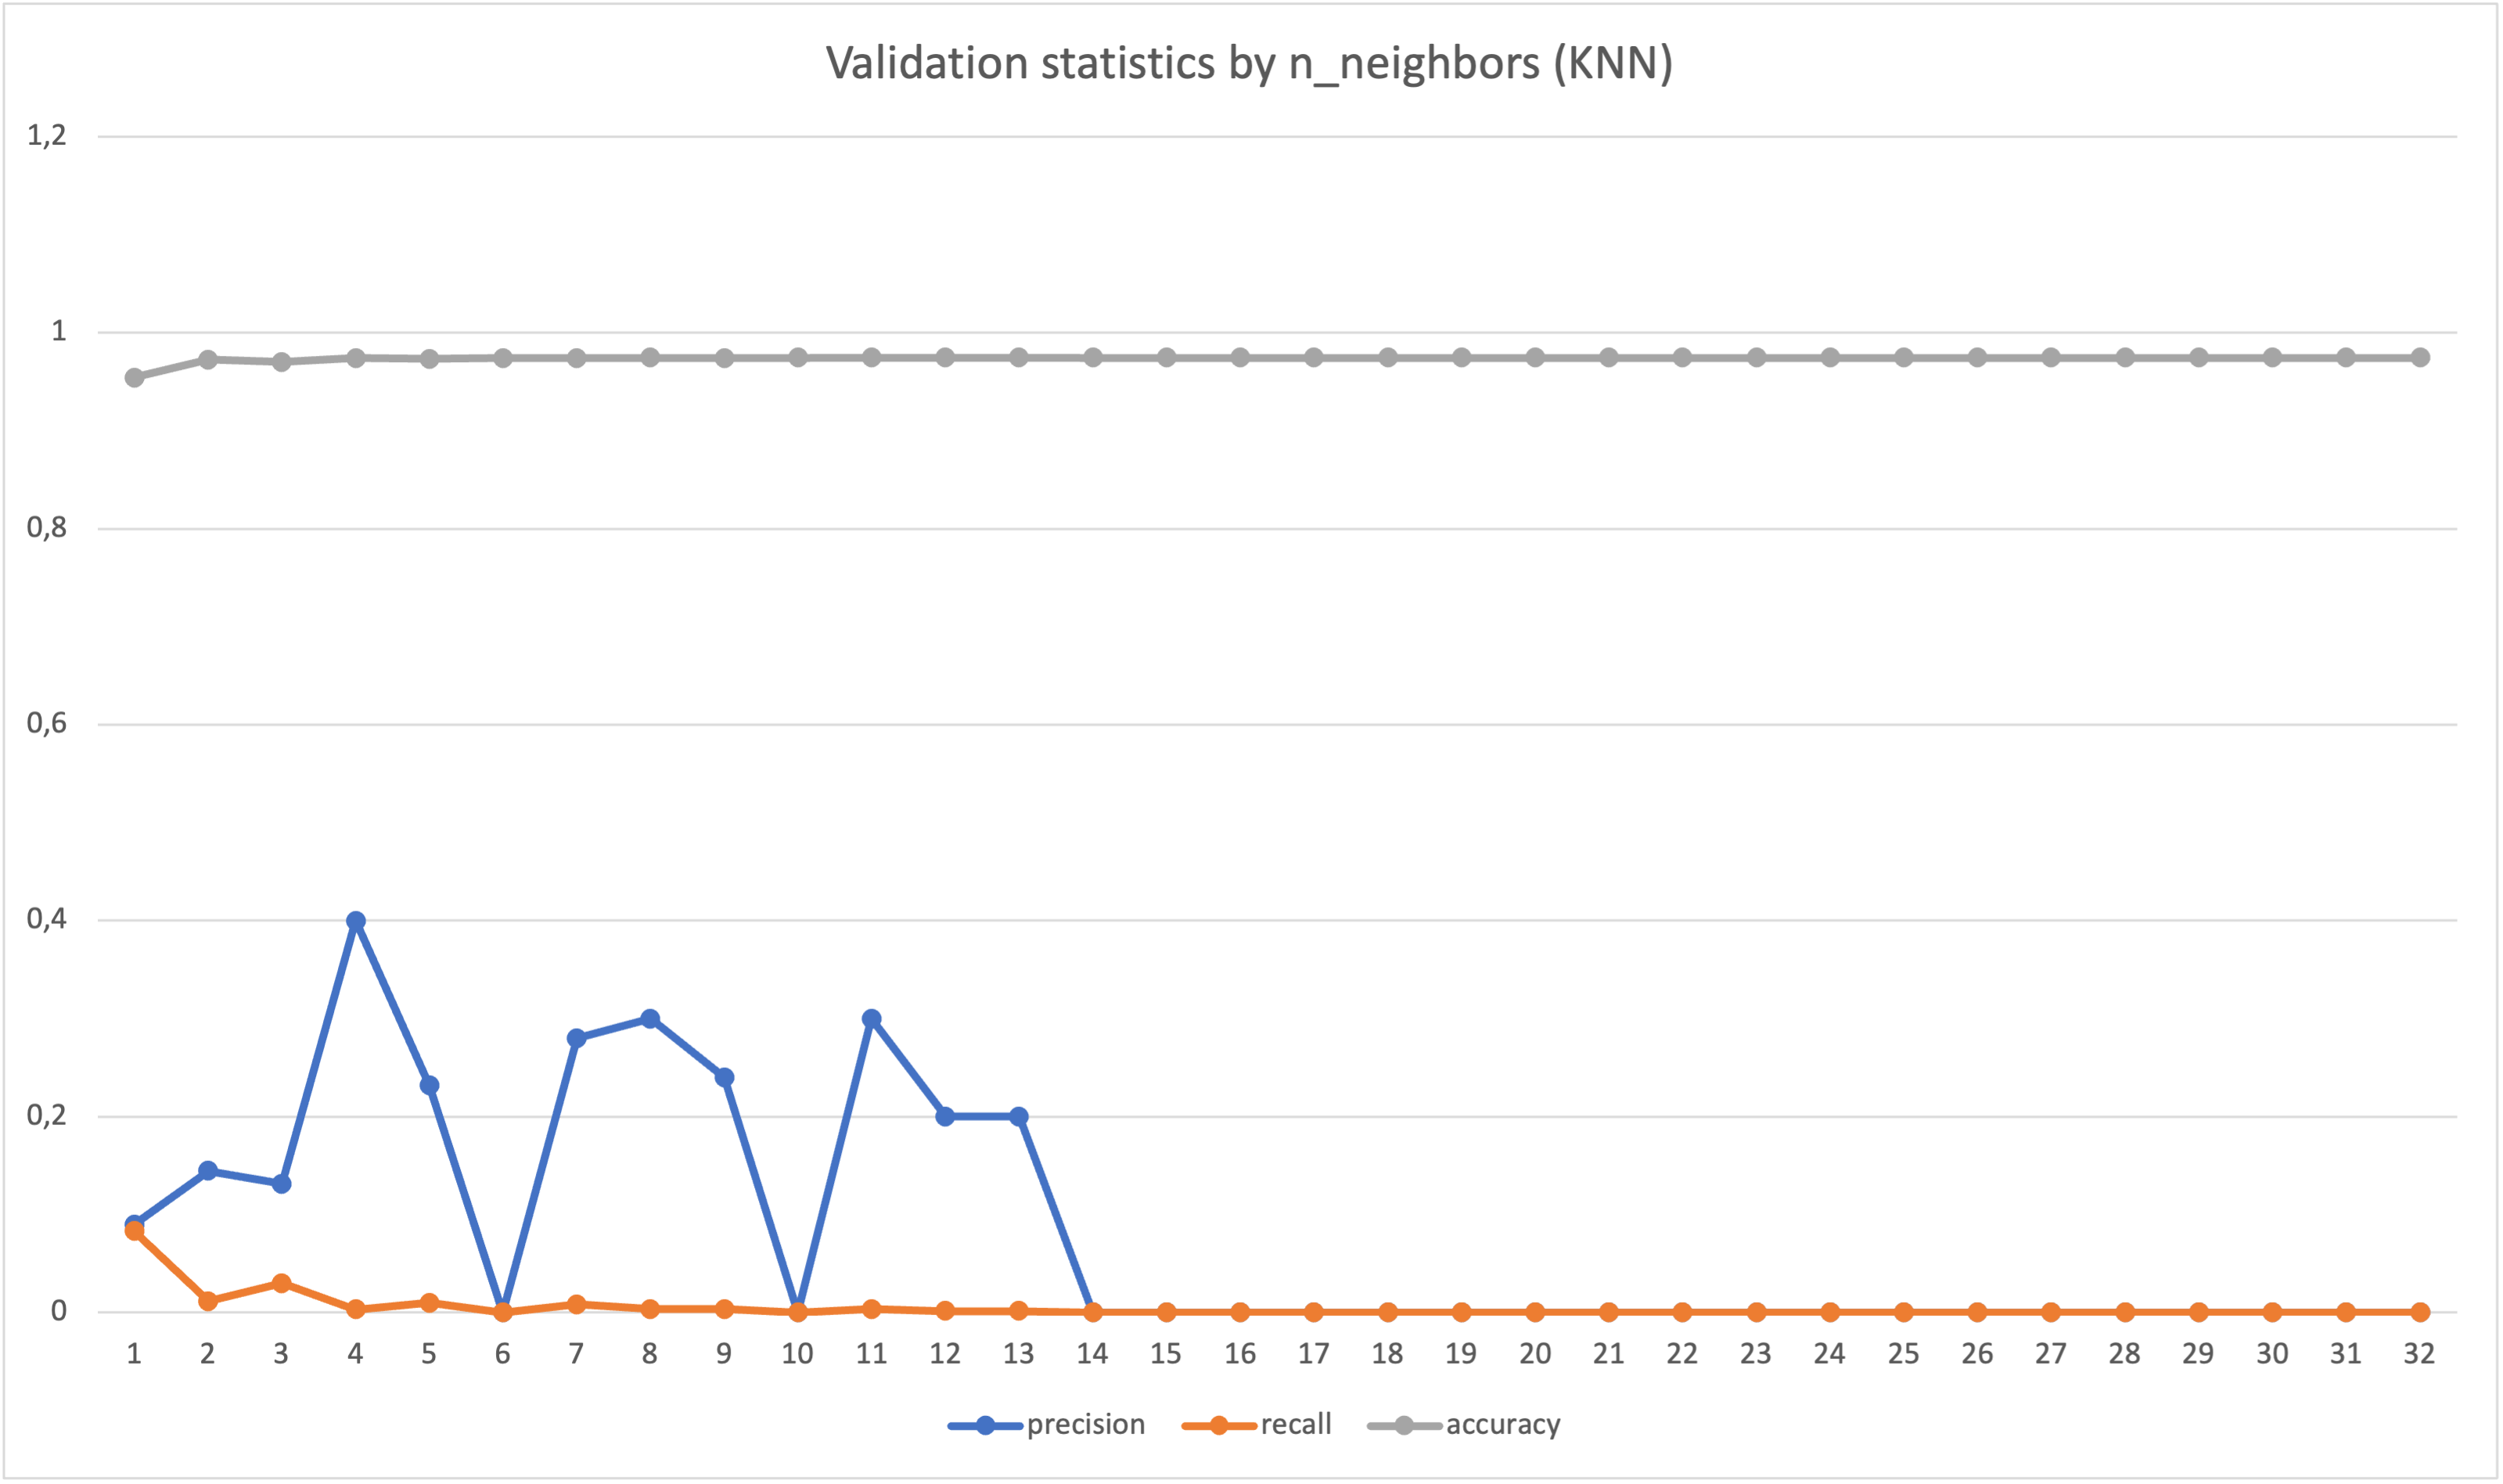
\includegraphics[width=0.49\columnwidth]{val_stats_n.png}
      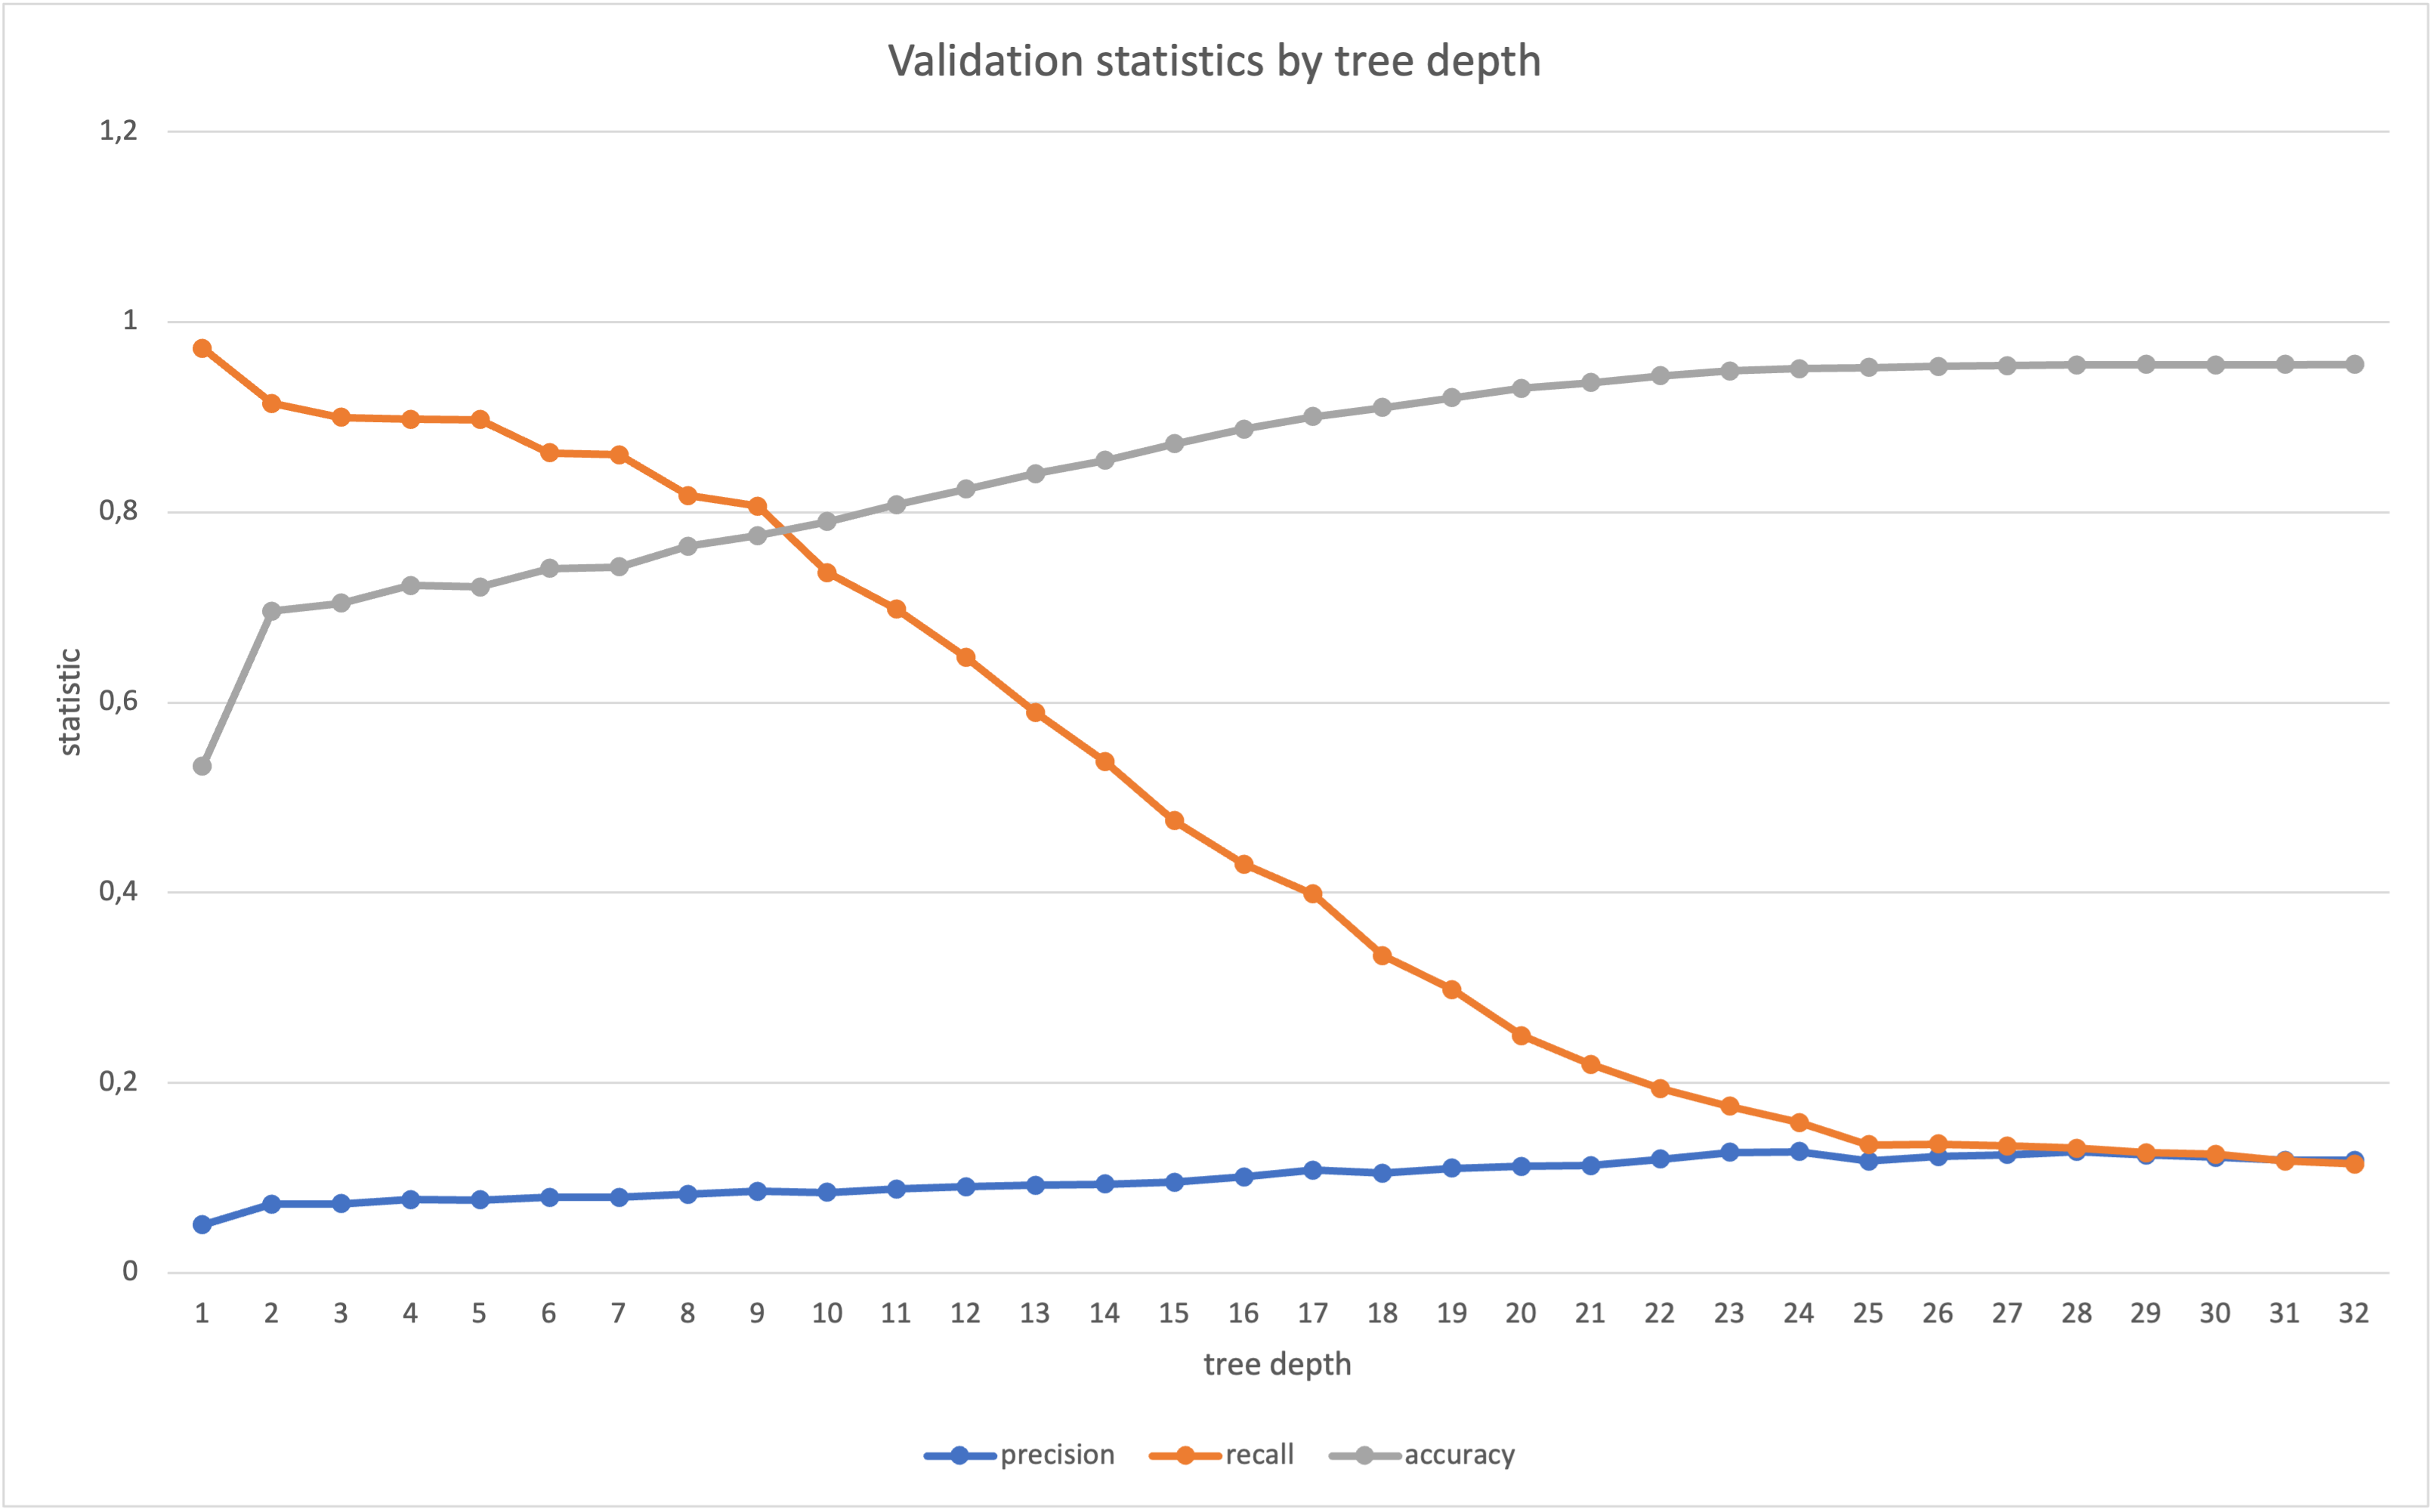
\includegraphics[width=0.49\columnwidth]{val_stats_dtc.png}
    \end{figure}
    As we see from the \autoref{fig:stats}, decision tree classifier models are more expectable, and perform better in the measured statistics.
    In decision tree classifier, the change of precision is minimal compared to recall, thus a suitable compromise between recall and accuracy is the decision
    tree classifier with tree depth 9. In the KNN context, the most promising parameter is the model with neighbor count 5, where the statistics are the best.
    \autoref{fig:results} represents an overview of these final candidates:
    \begin{table}[]
      \caption{Results of two machine learning methods}\label{fig:results}
      \centering
      \begin{tabular}{llll}
                           & Decision tree (max\_depth=9) & KNN (n\_neighbors=5) &  \\
      Training accuracy    & 0.78           & 0.97   &  \\
      Training precision   & 0.11           & 0.60   &  \\
      Training recall      & 0.99           & 0.058  &  \\
      Validation accuracy  & 0.78           & 0.97   &  \\
      Validation precision & 0.090          & 0.11  &  \\
      Validation recall    & 0.79           & 0.013 & 
      \end{tabular}
      \end{table}
    While KNN algorithm performs better in precision, we want to prioritize the slipping warning being 
    actually raised instead of the unconditional precision. Thus, recall is given more weight in this decision and
    the chosen method is the \textbf{decision tree classifier} with tree depth 9.

    Test set was simply split with \textit{train\_test\_split} function before the model training. 
    Test set size of 10\% was selected, as the amount of data was sufficiently low, so emphasis was based on training the model.
    Test errors for the selected method were: accuracy: 0.77, precision: 0.093, recall: 0.72.

    \section{Conclusions}
    Overall, the accuracy and recall statistics were good enough to suggest that it might be possible to predict 
    slipping conditions outside. Precision is still quite low, but that can be accepted as attention to safety is never irrelevant.

    While sufficient progress was achieved during the project, the result leaves space for improvement. Further
    study should be targeted specifically to improving the precision of the model. This might be done by continuing 
    hyperparameter tuning of the algorithms. One could also study if previous days' weather data would have an effect as new features.
    Until machine learning can replace the human consideration in this problem, we need to lean on the useful service
    which provided the data for this project.

    \newpage

    \begin{thebibliography}{9}
      \bibitem{warnsource}
      Slipping warning service API, \href{https://liukastumisvaroitus-api.beze.io/api/v1/warnings/}{https://liukastumisvaroitus-api.beze.io/api/v1/warnings/}
      \bibitem{fmisource}
      Finnish Metheorological Institute, observation history \href{https://en.ilmatieteenlaitos.fi/download-observations}{https://en.ilmatieteenlaitos.fi/download-observations}
    \end{thebibliography}

    \section{Appendices}
    \begin{itemize}
      \item Code and resources are available on the github page: \href{https://github.com/aksun1/cs-c3240-ml-project}{https://github.com/aksun1/cs-c3240-ml-project}.
    \end{itemize}


\end{document}